\documentclass{article}
\usepackage{cmap}
\usepackage[utf8]{inputenc}
\usepackage[english,ukrainian]{babel}
\usepackage{graphicx}
\usepackage{geometry}
\usepackage{listings}
\usepackage{float}
\usepackage{amsmath}
\usepackage{subfig}
\usepackage{xcolor}
\geometry{
	a4paper,
	left=20mm,
	right=20mm,
	top=15mm,
	bottom=15mm,
}
\lstset{
	tabsize=4,
	keepspaces,
	showstringspaces=false,
	escapeinside={(*@}{@*)},
	breaklines,
}
\graphicspath{ {./pictures} }
\setlength{\parindent}{4em}

\newcommand\subject{Архітектура комп'ютера}
\newcommand\lecturer{доцент кафедри ПЗ\\Крук О.Г.}
\newcommand\teacher{доцент кафедри ПЗ\\Крук О.Г.}
\newcommand\mygroup{ПЗ-22}
\newcommand\lab{10}
\newcommand\theme{Розроблення програми для арифметичного співпроцесора мікроконтролера Cortex-M4F}
\newcommand\purpose{Розвинути навики складання програми для арифметичного співпроцесора ARM-процесорів мовою асемблера для обчислення математичного виразу, відтранслювати і виконати в режимі відлагодження програму, складену відповідно до свого варіанту, обчислити заданий вираз в програмі мовою С та порівняти результати}

\begin{document}
	\begin{normalsize}
		\begin{titlepage}
			\thispagestyle{empty}
			\begin{center}
				\textbf{МІНІСТЕРСТВО ОСВІТИ І НАУКИ УКРАЇНИ\\
					НАЦІОНАЛЬНИЙ УНІВЕРСИТЕТ "ЛЬВІВСЬКА ПОЛІТЕХНІКА"}
			\end{center}
			\begin{flushright}
				\textbf{ІКНІ}\\
				Кафедра \textbf{ПЗ}
			\end{flushright}
			\vspace{200pt}
			\begin{center}
				\textbf{ЗВІТ}\\
				\vspace{10pt}
				до лабораторної роботи № \lab\\
				\textbf{на тему}: “\textit{\theme}”\\
				\textbf{з дисципліни}: “\subject”
			\end{center}
			\vspace{112pt}
			\begin{flushright}
				
				\textbf{Лектор}:\\
				\lecturer\\
				\vspace{28pt}
				\textbf{Виконав}:\\
				
				студент групи \mygroup\\
				Коваленко Д.М.\\
				\vspace{28pt}
				\textbf{Прийняв}:\\
				
				\teacher\\
				
				\vspace{28pt}
				«\rule{1cm}{0.15mm}» \rule{1.5cm}{0.15mm} 2022 р.\\
				$\sum$ = \rule{1cm}{0.15mm}……………\\
				
			\end{flushright}
			\vspace{\fill}
			\begin{center}
				\textbf{Львів — 2022}
			\end{center}
		\end{titlepage}
		
		\begin{description}
			\item[Тема.] \theme.
			\item[Мета.] \purpose.
		\end{description}
		
		\section*{Індивідуальне завдання}
		\begin{figure}[H]
			\centering
			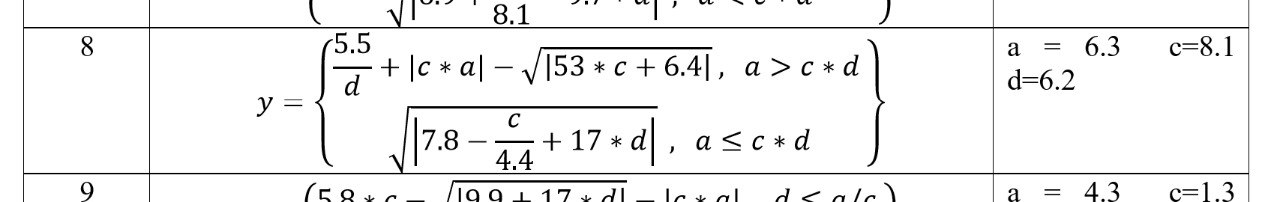
\includegraphics[scale=0.4]{v}
		\end{figure}
		
		\section*{Хід роботи}
		\subsection*{Код програми}
		\begin{lstlisting}
	AREA myCode, CODE, READONLY
MyProg
	EXPORT MyProg

	LDR r0, =a
	VLDM r0, {s0-s2}  ; s0=a, s1=c, s2=d
	LDR r0, =n1
	VLDM r0, {s7-s10}  ; n1, n2, n3, n4
	
	VMUL.F32 s3, s1, s2
	VCMP.F32 s0, s3
	VMRS APSR_nzcv, FPSCR
	BGT FIRST      ; a > c*d
	BLS SECOND      ; a <= c*d

FIRST
	VMOV.F32 s3, #5.5
	VDIV.F32 s3, s2
	
	VMUL.F32 s4, s1, s0
	VABS.F32 s4, s4
	
	VADD.F32 s3, s4    
	
	VMOV.F32 s3, r7    
	VMUL.F32 s4, s4, s1
	VMOV.F32 s3, r8
	VADD.F32 s4, s5
	VABS.F32 s4, s4
	VSQRT.F32 s4, s4
	
	VSUB.F32 s3, s4    
	
	LDR r0, =y      
	VSTM r0, {s3}
	B STOP

SECOND
	VMOV.F32 s3, s1
	VDIV.F32 s3, s10
	VSUB.F32 s9, s3
	VMOV.F32 s4, #17.0
	VMUL.F32 s4, s2
	VADD.F32 s4, s9
	VABS.F32 s4, s4
	VSQRT.F32 s3, s4
	
	LDR r0, =y      
	VSTM r0, {s3}

STOP B STOP
	a   DCFS 6.3
	c   DCFS 8.1
	d   DCFS 6.2
	
	n1  DCFS 6.4
	n2  DCFS 53.0
	n3  DCFS 7.8
	n4  DCFS 4.4

ALIGN
AREA MyData, DATA, ReadWrite

y   DCFS 0.0
	END
		\end{lstlisting}

\begin{figure}[H]
	\centering
	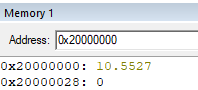
\includegraphics[scale=0.7]{1}
	\caption{Результат обчислення}
\end{figure}

\section*{Код програми (С)}			
\begin{lstlisting}
#include <stdio.h>
#include <stdlib.h>
#include <math.h>

int main() {
	float a = 6.3;
	float c = 8.1;
	float d = 6.2;
	
	if (a > c*d) {
		float res = 5.5/d + abs(c*a) - sqrt(abs(53.0*c + 6.4));
		printf("%f\n", res);
	} else if (a <= c*d) {
		float res = sqrt(abs(7.8-c/4.4+17*d));
		printf("%f\n", res);
	}
}
\end{lstlisting}


\begin{figure}[H]
	\centering
	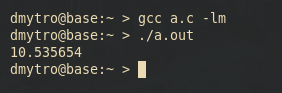
\includegraphics[scale=0.7]{2}
	\caption{Результат обчислення (С)}
\end{figure}
			
		\section*{Висновки}
		Під час виконання лабораторної роботи я розвинув навики складання програми для арифметичного співпроцесора ARM-процесорів мовою асемблера для обчислення математичного виразу, відтранслював і виконав в режимі відлагодження програму, складену відповідно до свого варіанту, обчислив заданий вираз в програмі мовою С та порівняв результати.
		
	\end{normalsize}
\end{document}